\documentclass{article}
\usepackage{algorithm}
\usepackage{algpseudocode}
\usepackage{graphicx}
\graphicspath{ {images/} }
\usepackage{amssymb}
\usepackage{adjustbox}

\begin{document}
		
\begin{algorithm}
\caption{Reverse-Cuthill-McGee Redordering}\label{RCM}
\begin{algorithmic}
\Procedure{RCM}{$mesh$}
	\State node\_label $\gets$ num\_nodes$ + 1$
	\State face\_label $\gets$ num\_faces$ + 1$
	\State Queue q
	\State MeshEntity start\_entity $\gets$ mesh.getStartNode()
	\State q.enqueue(start\_entity)
	\While{q.size() $> 0$}

	\EndWhile


\EndProcedure
\State

\Procedure{getStartNode}{$mesh$}
	\State\Comment{for $M^{0}_{i} \in [M^{0}]$ \textbf{and}\  $M^{0}_{i} \sqsubset G^{0}$ find min $M^{0}_{i}\{M^{1}\}$}
	\State min\_order $\gets$ INTMAX
	\State MeshEntity best\_vertex
	\State MeshEntity entity $\gets$ mesh.getFirstVertex()
	\While{vertex $\gets$ mesh.getNextVertex()}
		\If{mesh.getModelType(vertex) == MODEL\_VERTEX}
			\State adjacency\_size $\gets$ mesh.getAdjacent()
			\If{adjaceny\_size $<$ min\_order}
				\State min\_order $\gets$ adjaceny\_size
				\State best\_vertex $\gets$ entity
			\EndIf
		\EndIf
	\EndWhile
	\State\Return best\_entity
\EndProcedure

\end{algorithmic}
\end{algorithm}

\begin{figure}[h]
\caption{Original labeling of entities by memory address order}
\adjustbox{trim= {0.2\width} {0} {0.2\width} {0}, clip}
{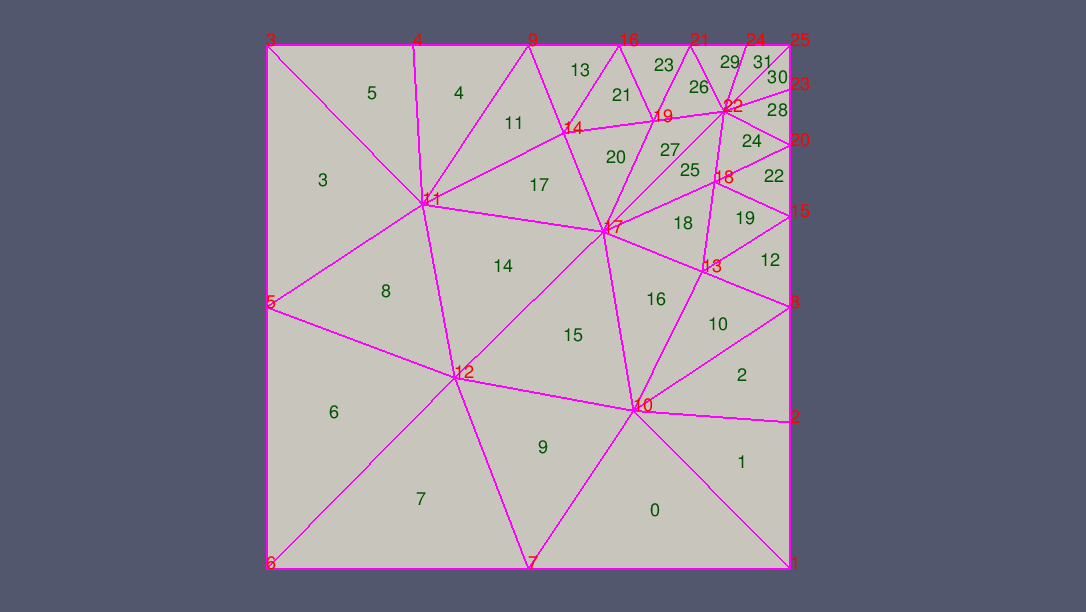
\includegraphics[width = 15cm ]{pre_b}}
\centering
\end{figure}

\begin{figure}[h]
\caption{Reordering with Reverse Cuthill-McGee}
\adjustbox{trim= {0.2\width} {0} {0.2\width} {0}, clip}
{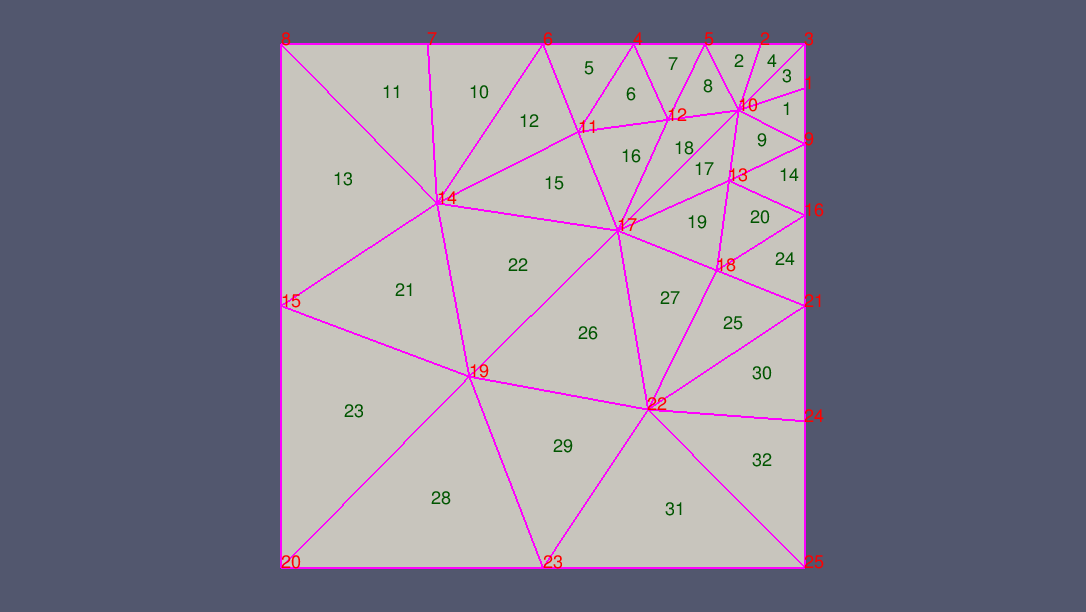
\includegraphics[width = 15cm ]{post_b}}
\centering
\end{figure}

\begin{figure}[h]
\caption{Original labeling of entities by memory address order}
\adjustbox{trim= {0.2\width} {0} {0.2\width} {0}, clip}
{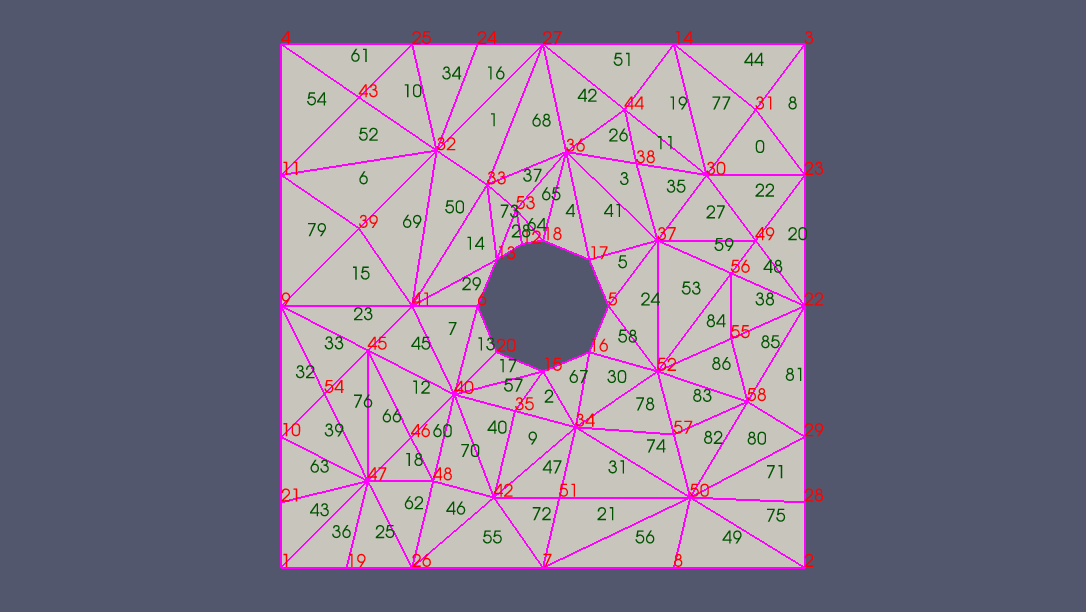
\includegraphics[width = 15cm ]{pre_c}}
\centering
\end{figure}

\begin{figure}[h]
\caption{Reordering with Reverse Cuthill-McGee}
\adjustbox{trim= {0.2\width} {0} {0.2\width} {0}, clip}
{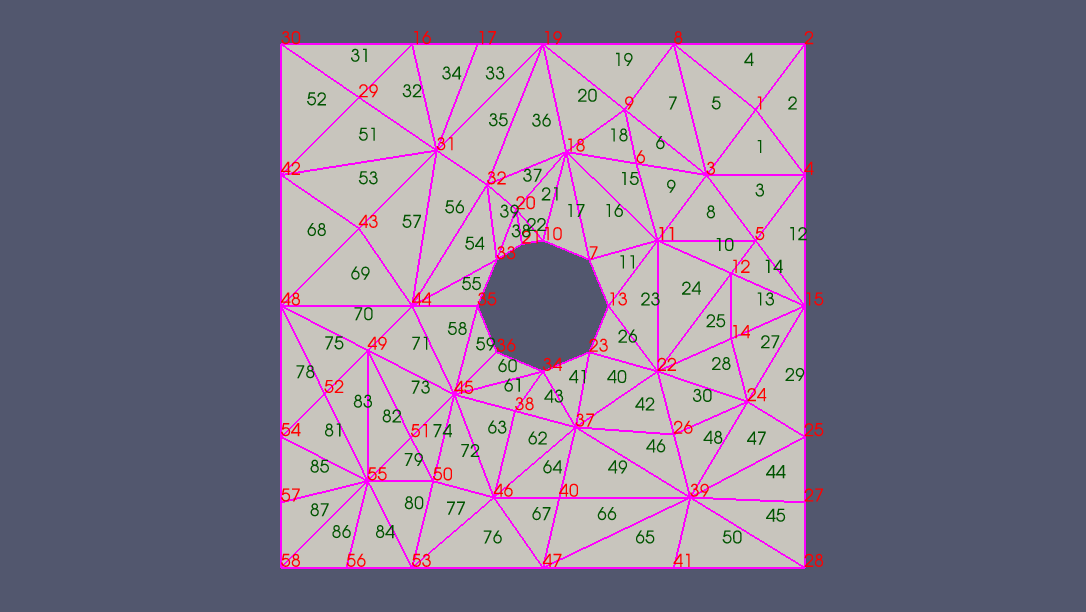
\includegraphics[width = 15cm ]{post_c}}
\centering
\end{figure}

\begin{figure}[h]
\caption{Original labeling of entities by memory address order}
\adjustbox{trim= {0.2\width} {0} {0.2\width} {0}, clip}
{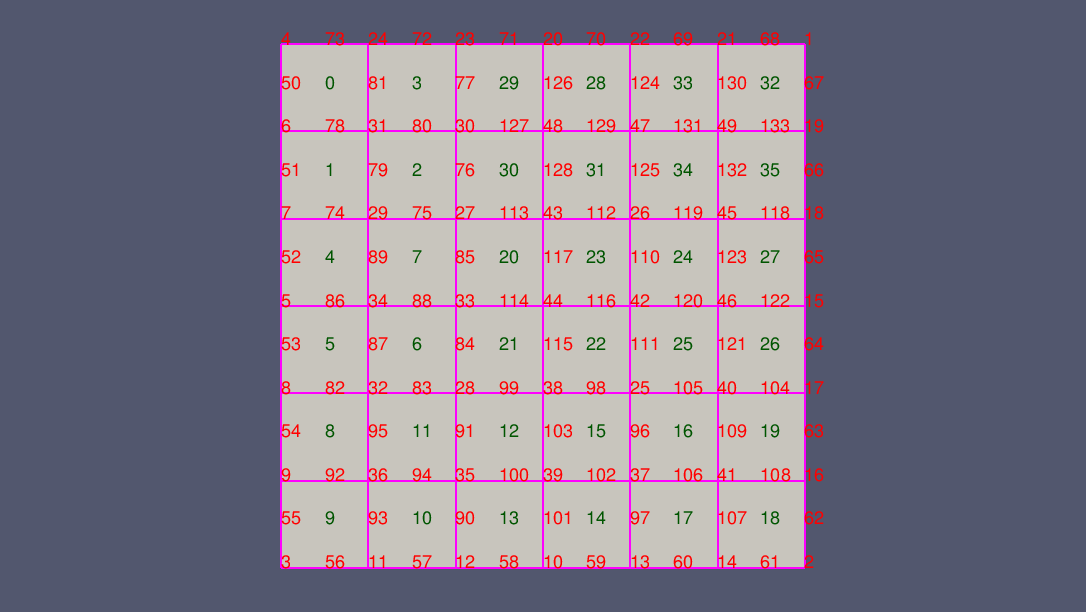
\includegraphics[width = 15cm ]{pre_a}}
\centering
\end{figure}

\begin{figure}[h]
\caption{Reordering with Reverse Cuthill-McGee}
\adjustbox{trim= {0.2\width} {0} {0.2\width} {0}, clip}
{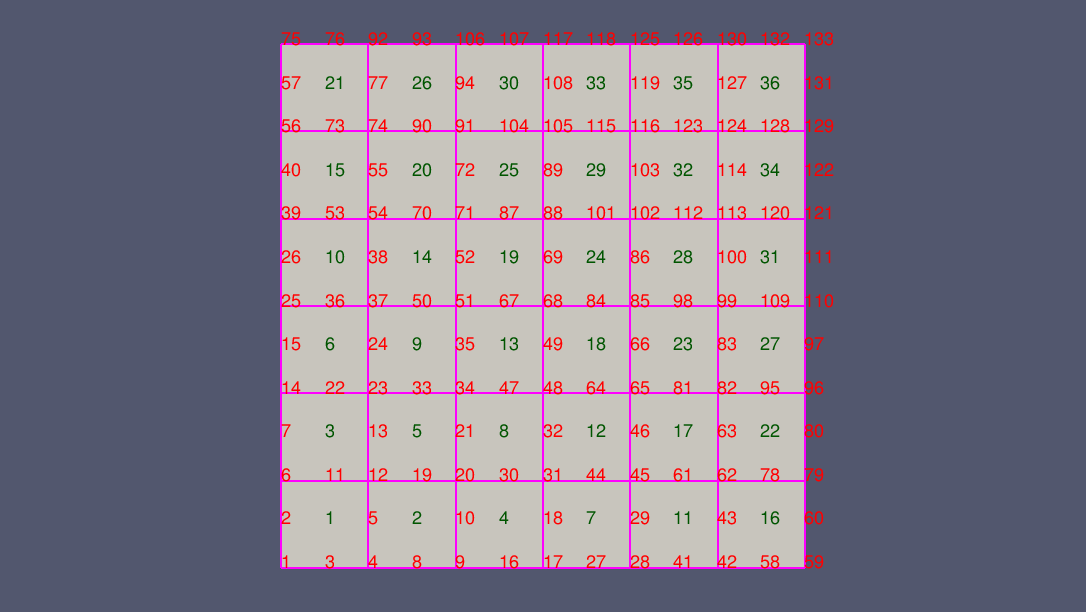
\includegraphics[width = 15cm ]{post_a}}
\centering
\end{figure}

\end{document}